% =====================================================================
% 5. Area 3: generative AI (PRDL, Maria Martinez)
% Oriana's block (T23; DECISIONS D13, D19; block note 13), summarised and
% attributed; reviewed by Maria.
% =====================================================================
\section{Area 3: generative AI (Oriana's block, summarised)}\label{sec:generative}

The third area asks at least for an autoregressive sequence generator, RNN or Transformer based, like the
small LLM-style models of the course \cite{course_message_2011}. This block was designed, run and
analysed by Oriana; I reviewed it. It reuses my hand-written attention module with a causal mask, which
is why I summarise it here with the points that connect to my blocks.

\paragraph{Model.} Lead II is turned into a sequence of discrete symbols, like the characters of the class
text-generation notebooks \cite{course_nb_sampling}: each sample is quantised on a uniform grid of
microvolts over a fixed range (\generativeVocabBase{} levels of \generativeDeltaUvBase\,\textmu V in the
baseline; 64 and 2560 levels as ablations). Representing amplitude ranges by discrete symbols is also the
idea of recent token-based ECG models \cite{han2025ecgbyte}. The ECG-GPT is a decoder-only Transformer, the
architecture of GPT, a ``decoder-only transformer with masked self-attention heads''
\cite{radford2018improving}, trained with the standard language-modelling objective of predicting each
token from the previous ones \cite{radford2018improving}; an LSTM of the same size was trained on the same
data and budget. The causal mask sets the attention to future tokens to zero, so the whole window is
trained in parallel while each position only sees the past. Non-uniform (mu-law) quantisation was not
tried.

\paragraph{Metric.} The cross-entropy per token cannot compare vocabularies: with fewer, wider levels each
prediction is easier, so its cross-entropy is lower even if the model describes the signal worse.
Oriana's block therefore reports bits per sample, $(\mathrm{CE} + \ln \Delta)/\ln 2$ with $\Delta$ the
width of a level in microvolts: the cost of coding the microvolt value of the next sample if every value
inside a level is equally likely, which can be compared whatever the vocabulary. Entropy in bits per symbol has been used before to report character-level models
\cite{pascanu2013difficulty}; the correction for the level width is our own argument.

\paragraph{Main findings} (Table~\ref{tab:generative_ablations}).
\begin{itemize}[leftmargin=1.2em,itemsep=2pt]
  \item Every generator beats a counting bigram model; the baseline codes the signal in
        \generativeBitsMeanBase{} bits per sample against \generativeBigramBitsVTwoFiveSix{} for the bigram.
  \item The model with the finest levels (\generativeVocabVocabTwoFiveSixZero{} levels of
        \generativeDeltaUvVocabTwoFiveSixZero\,\textmu V) needs the fewest bits
        (\generativeDiffMeanVocabTwoFiveSixZero{} with respect to the baseline) and became the pre-trained
        model of Section~\ref{sec:strategies}. The LSTM (\generativeDiffMeanLstm{}) and a context of 5\,s
        (\generativeDiffMeanCtxFiveZeroZero{}) also improve on the baseline, in all seeds.
  \item \textbf{Positional encoding matters for generation:} without it the cost rises by
        \generativeDiffMeanNoPos{} bits per sample. This is the opposite of my Transformer classifier, where
        removing it helped (Section~\ref{sec:transformer}). The contrast is consistent: a classifier of
        beat shapes can work on a set of patches, but predicting the next sample requires knowing where in
        the beat the model is. Causal language models without explicit positions have been found to remain
        competitive \cite{haviv2022transformer}; our setting (a periodic signal and a very small model) is
        different, and why positions matter here is a hypothesis of Oriana's block.
  \item Without the causal mask the training loss falls almost to zero because the model reads the answer,
        but at the only position whose target is not in its input it is worse than the baseline, and its
        samples are poor: the mask is what makes parallel training honest.
  \item Decoding matters as much as the model (Figure~\ref{fig:generative_samples}): greedy decoding
        collapses to a flat line in every record, temperatures around 0.8--1.0 give realistic beats, and a
        high temperature gives noise. Top-$k$ sampling, which samples ``from the k = 10 most likely
        candidates'' \cite{fan2018hierarchical}, becomes almost greedy with 2560 levels, because ten levels
        of 1\,\textmu V are a very narrow band.
\end{itemize}
Oriana's block states two limits that I keep: every generator stopped at the 50-epoch limit without
converging, so the comparisons are at equal budget; and the comparison of context lengths is at equal
epochs, not at equal number of samples seen. The interpretations of the cost against context (the model
using the previous beat) and of the attention maps are hypotheses of that block.

% Shared float (common/make_floats.py). Table: tables/generative_ablations.tex
\begin{table}[htbp]
\centering
\caption[Generators: ablations (validation)]{Generators of lead II on the validation fold (mean $\pm$ SD over seeds 42--44). CE: cross-entropy per token (nats), not comparable across vocabularies; bits per sample: comparable; $\Delta$ bits: mean paired difference with the baseline (negative = better). The model without the causal mask is not compared (it sees its target).}
\label{tab:generative_ablations}
\small
\begin{adjustbox}{max width=\textwidth}
% Generated by src/generative_experiments.py from results/logs/generative_summary.json.
% Needs report/numbers.tex (alias "generative" in report/runs.json) and \usepackage{booktabs}. Wide: use \resizebox{\textwidth}{!}{...}.
% CE: validation cross-entropy per token (nats); it depends on the vocabulary. Bits: bits per sample, comparable across vocabularies.
% Delta: paired difference in bits with the baseline, same seed; negative = fewer bits. Last: CE at the last position of the window.
\begin{tabular}{llrrrccccr}
\toprule
Factor & Configuration & Parameters & $L$ & $V$ & CE (nats) & Bits per sample & $\Delta$ bits & Seeds better / worse & Last-position CE \\
\midrule
baseline & ECG-GPT: causal Transformer, 2 blocks, $L$ = 250, $V$ = 256 & \generativeParamsBase{} & \generativeContextBase{} & \generativeVocabBase{} & \generativeCeMeanBase{} $\pm$ \generativeCeSdBase{} & \generativeBitsMeanBase{} $\pm$ \generativeBitsSdBase{} & --- & --- & \generativeCeLastMeanBase{} \\
\addlinespace
architecture & LSTM, 2 layers of 160 (same size) & \generativeParamsLstm{} & \generativeContextLstm{} & \generativeVocabLstm{} & \generativeCeMeanLstm{} $\pm$ \generativeCeSdLstm{} & \generativeBitsMeanLstm{} $\pm$ \generativeBitsSdLstm{} & \generativeDiffMeanLstm{} & \generativeNSeedsBetterLstm{} / \generativeNSeedsWorseLstm{} of \generativeNSeedsComparedLstm{} & \generativeCeLastMeanLstm{} \\
\addlinespace
context length & Context of 100 samples (1 s) & \generativeParamsCtxOneZeroZero{} & \generativeContextCtxOneZeroZero{} & \generativeVocabCtxOneZeroZero{} & \generativeCeMeanCtxOneZeroZero{} $\pm$ \generativeCeSdCtxOneZeroZero{} & \generativeBitsMeanCtxOneZeroZero{} $\pm$ \generativeBitsSdCtxOneZeroZero{} & \generativeDiffMeanCtxOneZeroZero{} & \generativeNSeedsBetterCtxOneZeroZero{} / \generativeNSeedsWorseCtxOneZeroZero{} of \generativeNSeedsComparedCtxOneZeroZero{} & \generativeCeLastMeanCtxOneZeroZero{} \\
\addlinespace
vocabulary & 64 levels of 40 $\mu$V & \generativeParamsVocabSixFour{} & \generativeContextVocabSixFour{} & \generativeVocabVocabSixFour{} & \generativeCeMeanVocabSixFour{} $\pm$ \generativeCeSdVocabSixFour{} & \generativeBitsMeanVocabSixFour{} $\pm$ \generativeBitsSdVocabSixFour{} & \generativeDiffMeanVocabSixFour{} & \generativeNSeedsBetterVocabSixFour{} / \generativeNSeedsWorseVocabSixFour{} of \generativeNSeedsComparedVocabSixFour{} & \generativeCeLastMeanVocabSixFour{} \\
\addlinespace
positional encoding & No positional encoding & \generativeParamsNoPos{} & \generativeContextNoPos{} & \generativeVocabNoPos{} & \generativeCeMeanNoPos{} $\pm$ \generativeCeSdNoPos{} & \generativeBitsMeanNoPos{} $\pm$ \generativeBitsSdNoPos{} & \generativeDiffMeanNoPos{} & \generativeNSeedsBetterNoPos{} / \generativeNSeedsWorseNoPos{} of \generativeNSeedsComparedNoPos{} & \generativeCeLastMeanNoPos{} \\
\addlinespace
causal mask & No causal mask (sees the future) & \generativeParamsNoMask{} & \generativeContextNoMask{} & \generativeVocabNoMask{} & \generativeCeMeanNoMask{} $\pm$ \generativeCeSdNoMask{} & \generativeBitsMeanNoMask{} $\pm$ \generativeBitsSdNoMask{} & --- & --- & \generativeCeLastMeanNoMask{} \\
\addlinespace
vocabulary & 2560 levels of 1 $\mu$V (lossless) & \generativeParamsVocabTwoFiveSixZero{} & \generativeContextVocabTwoFiveSixZero{} & \generativeVocabVocabTwoFiveSixZero{} & \generativeCeMeanVocabTwoFiveSixZero{} $\pm$ \generativeCeSdVocabTwoFiveSixZero{} & \generativeBitsMeanVocabTwoFiveSixZero{} $\pm$ \generativeBitsSdVocabTwoFiveSixZero{} & \generativeDiffMeanVocabTwoFiveSixZero{} & \generativeNSeedsBetterVocabTwoFiveSixZero{} / \generativeNSeedsWorseVocabTwoFiveSixZero{} of \generativeNSeedsComparedVocabTwoFiveSixZero{} & \generativeCeLastMeanVocabTwoFiveSixZero{} \\
\addlinespace
context length & Context of 500 samples (5 s) & \generativeParamsCtxFiveZeroZero{} & \generativeContextCtxFiveZeroZero{} & \generativeVocabCtxFiveZeroZero{} & \generativeCeMeanCtxFiveZeroZero{} $\pm$ \generativeCeSdCtxFiveZeroZero{} & \generativeBitsMeanCtxFiveZeroZero{} $\pm$ \generativeBitsSdCtxFiveZeroZero{} & \generativeDiffMeanCtxFiveZeroZero{} & \generativeNSeedsBetterCtxFiveZeroZero{} / \generativeNSeedsWorseCtxFiveZeroZero{} of \generativeNSeedsComparedCtxFiveZeroZero{} & \generativeCeLastMeanCtxFiveZeroZero{} \\
\midrule
\multicolumn{10}{l}{\emph{Baselines without training (bits per sample on the same validation records)}} \\
\multicolumn{6}{l}{Uniform over the range} & \generativeUniformBits{} & & & \\
\multicolumn{6}{l}{Unigram / bigram counts, $V$ = 64} & \generativeUnigramBitsVSixFour{} / \generativeBigramBitsVSixFour{} & & & \\
\multicolumn{6}{l}{Unigram / bigram counts, $V$ = 256} & \generativeUnigramBitsVTwoFiveSix{} / \generativeBigramBitsVTwoFiveSix{} & & & \\
\multicolumn{6}{l}{Unigram / bigram counts, $V$ = 2560} & \generativeUnigramBitsVTwoFiveSixZero{} / \generativeBigramBitsVTwoFiveSixZero{} & & & \\
\bottomrule
\end{tabular}

\end{adjustbox}
\end{table}

% Shared float (common/make_floats.py). Figure: figures/generative_samples.pdf
\begin{figure}[htbp]
\centering
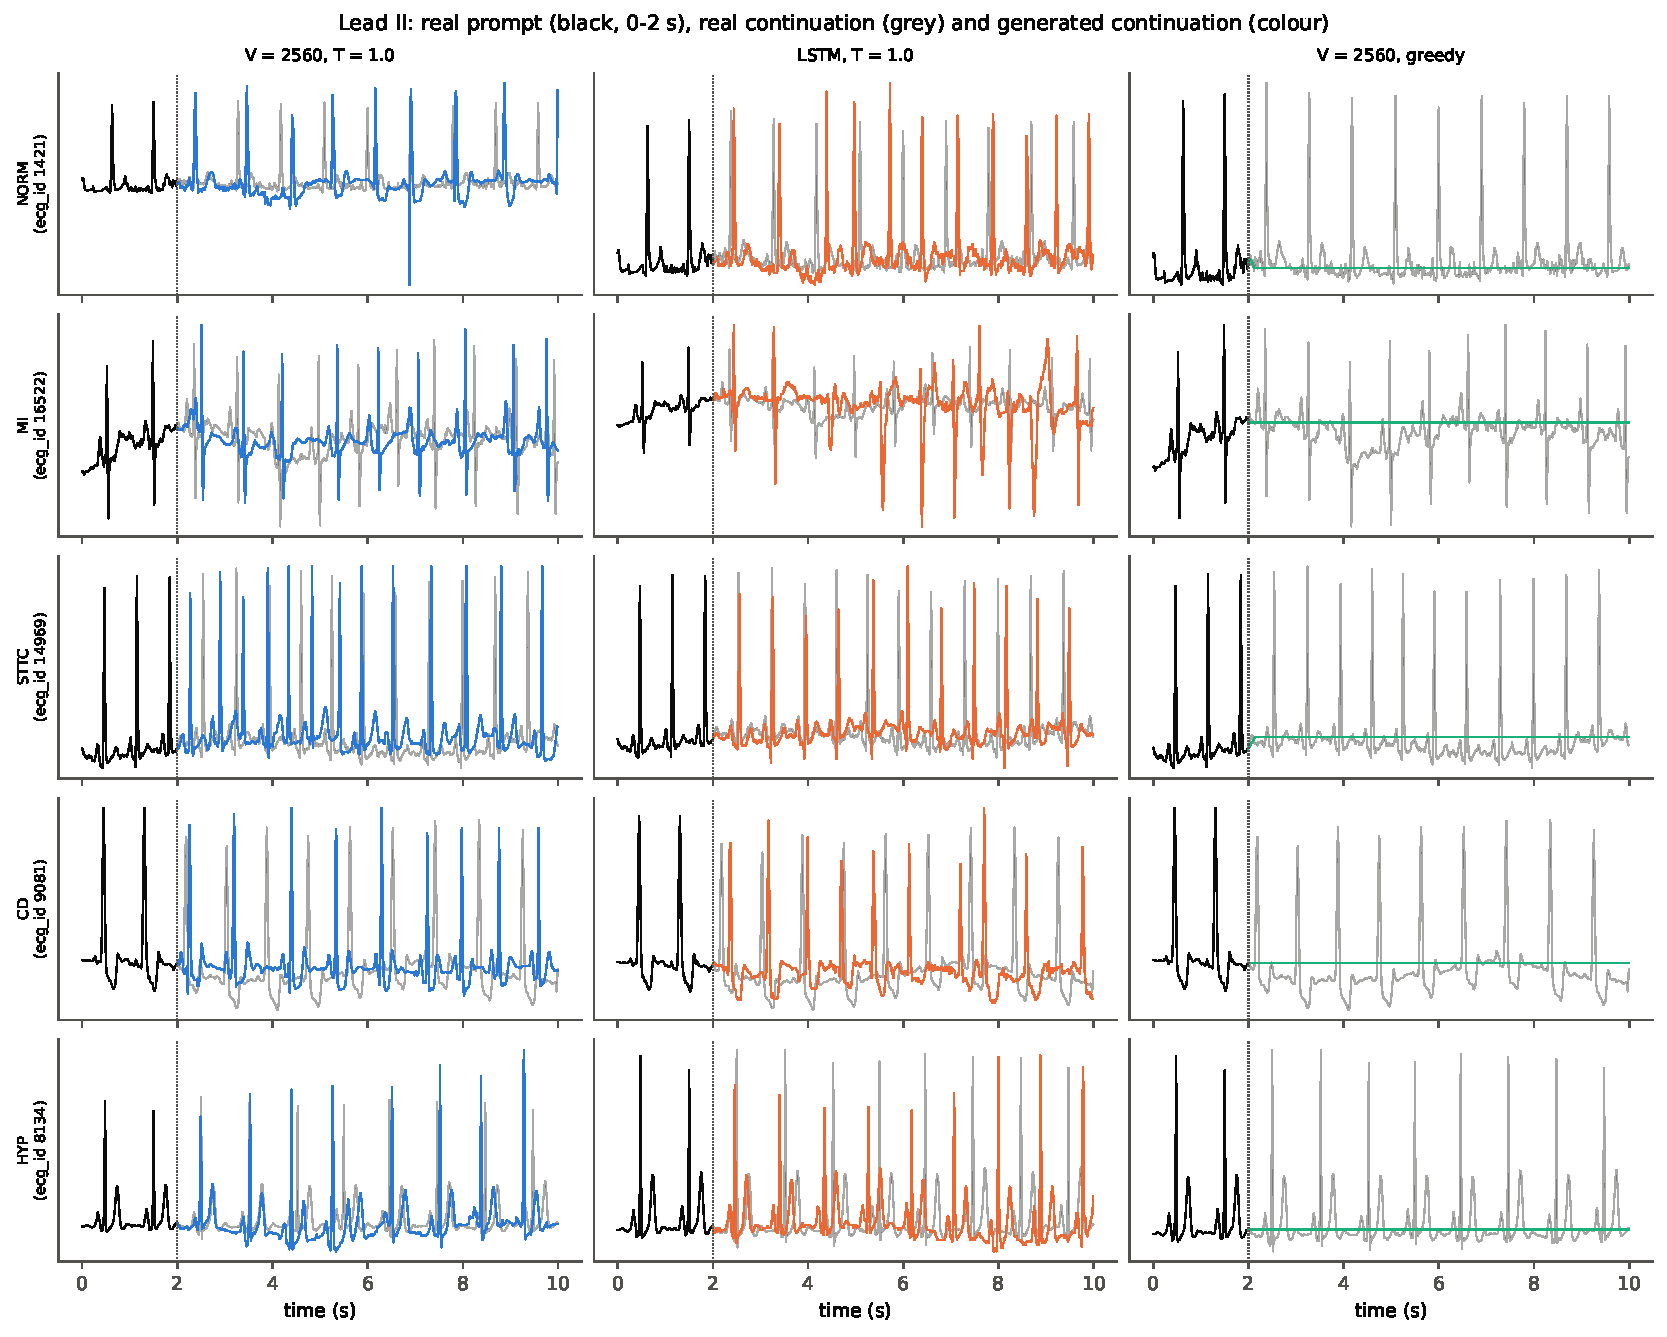
\includegraphics[width=\textwidth,height=0.42\textheight,keepaspectratio]{figures/generative_samples.pdf}
\caption[Generators: real and generated lead II]{Lead II of one validation record per superclass: real 2\,s prompt (black), real continuation (grey) and generated continuation (colour) of the selected ECG-GPT ($V = 2560$, $T = 1$), the LSTM ($T = 1$) and the ECG-GPT with greedy search.}
\label{fig:generative_samples}
\end{figure}

